\section{Penyelesaian Soal Nomor 2: Segmentasi Karakter}
\label{sec:soal2}

\subsection{Tujuan dan data masukan}
Bagian ini dikerjakan oleh Dustin Pranata Wangsawidjaja. Program
\path{soal2/main.py} memisahkan karakter pada citra teks menjadi gambar
individual dengan bantuan \kode{regionprops}~\cite{soal-uts,skimage-regions}.
Tujuannya adalah segmentasi karakter, bukan pengenalan huruf atau OCR.
Citra \path{soal2/teks.png} memuat ZEUS, TWINPEAK, dan ACOSTA, dengan
total acuan 18 karakter. Karakter terang berada pada latar gelap, saling
terpisah, dan mempunyai orientasi yang bervariasi.

\subsection{Segmentasi dan penggunaan regionprops}
Citra berwarna diubah menjadi grayscale; masukan satu kanal dinormalisasi
dengan membagi intensitas terhadap nilai maksimum. Ambang Otsu menghasilkan
mask \(B=[I>t]\). Jika lebih dari setengah piksel mask bernilai benar,
mask dibalik agar karakter menjadi foreground. Objek dengan luas kurang
dari 10 piksel dihapus menggunakan \kode{remove_small_objects}, kemudian
\kode{measure.label} memakai konektivitas 8 untuk memberi identitas pada
setiap komponen. Nilai luas minimum merupakan parameter implementasi,
bukan ketentuan tetap untuk semua resolusi citra.

\begin{table}[H]
\centering
\caption{Peran atribut regionprops pada segmentasi karakter.}
\begin{tabularx}{\textwidth}{@{}lX@{}}
\toprule
\textbf{Atribut} & \textbf{Penggunaan}\\
\midrule
\kode{bbox} & Kotak pembatas untuk penyaringan border dan visualisasi.\\
\kode{image} & Mask milik region saja untuk gambar karakter individual.\\
\kode{centroid} & Titik pusat untuk pengelompokan baris dan pengurutan.\\
\bottomrule
\end{tabularx}
\end{table}

Region dipertahankan apabila tinggi kotak pembatasnya kurang dari setengah
tinggi citra dan lebarnya kurang dari setengah lebar citra. Penyaringan
ini menghapus garis border yang membentuk komponen besar. Aturan tersebut
berdasarkan dimensi \emph{bounding box}, bukan berdasarkan luas region.

Mask \kode{region.image} dipakai agar piksel huruf tetangga yang mungkin
masuk ke kotak pembatas huruf miring tidak ikut tersimpan. Setiap mask
diubah menjadi citra biner 0/255 dan diberi margin hitam tiga piksel.
Orientasi huruf dipertahankan; program tidak memutar huruf menjadi tegak.

\clearpage
\subsection{Pengurutan dan kode semu}
RANSAC dengan \kode{LineModelND} mengelompokkan centroid yang mendekati
satu garis. Ambang jarak adalah \(0{,}045\max(H,W)\), dengan dua sampel
minimum dan paling banyak 2000 percobaan. Kelompok baris diurutkan menurut
rata-rata koordinat vertikal, kemudian karakter pada setiap baris diurutkan
dari kiri ke kanan. Sisa satu atau dua objek menjadi satu kelompok terakhir.
Prosedur ini mengatur urutan berkas; pemisahan karakter tetap ditentukan
oleh komponen terhubung dan \kode{regionprops}.

\noindent\begin{minipage}{\textwidth}
\begin{lstlisting}[style=pseudocode,caption={Alur segmentasi karakter pada program Dustin.}]
INPUT citra teks, luas_min = 10, padding = 3
G = grayscale dan normalisasi citra
B = (G > ambang_otsu(G))
IF rata-rata B > 0.5: B = komplemen B
B = hapus_objek_kecil(B, luas_min)
L = label_8_tetangga(B)
R = regionprops(L)
Pertahankan region dengan tinggi bbox < H/2
dan lebar bbox < W/2
Kelompokkan centroid R ke baris menggunakan RANSAC
Urutkan baris atas-ke-bawah, karakter kiri-ke-kanan
FOR region dalam urutan:
    C = uint8(region.image * 255)
    C = tambah_margin_hitam(C, padding)
    Simpan C sebagai karakter_XX.png
OUTPUT gambar karakter dan visualisasi bbox
\end{lstlisting}
\end{minipage}

\subsection{Batasan metode}
Karakter bersentuhan dapat menjadi satu komponen, sedangkan karakter dengan
bagian terpisah, seperti titik dan batang pada huruf i, dapat menjadi beberapa
objek. Pengurutan mengasumsikan baris kira-kira lurus dan tidak vertikal.
Ambang global dan aturan dimensi border perlu disesuaikan bila latar,
resolusi, atau ukuran karakter berubah. Hasil yang dilaporkan berlaku pada
citra masukan yang disertakan; program tidak mengklasifikasikan identitas huruf.

\clearpage
\subsection{Hasil dan pemeriksaan}
Eksekusi ulang menghasilkan 18 karakter, sesuai jumlah yang terlihat pada
citra: ZEUS sebanyak 4, TWINPEAK sebanyak 8, dan ACOSTA sebanyak 6.
Berkas \kode{karakter_01.png} sampai \kode{karakter_18.png} tersimpan
pada \path{soal2/hasil_karakter/}. Visualisasi kotak pembatas ditunjukkan
pada Gambar~\ref{fig:karakter-bbox}.

\begin{figure}[H]
\centering
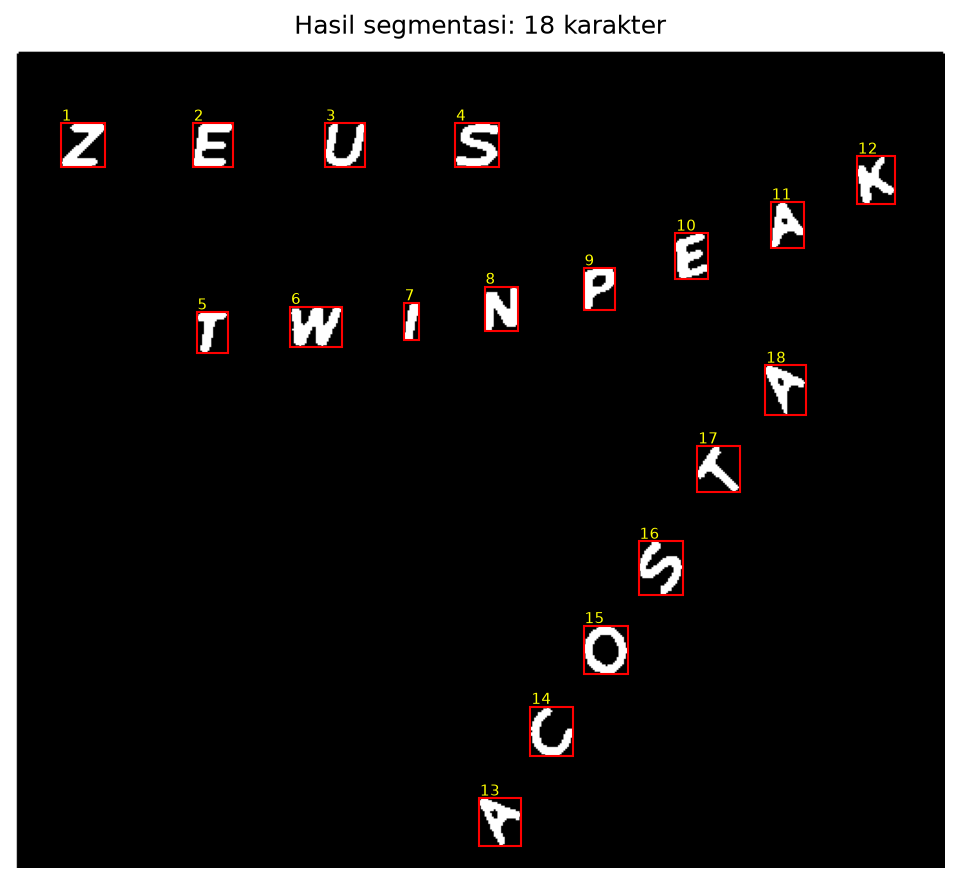
\includegraphics[width=0.65\textwidth,height=0.37\textheight,keepaspectratio]{images/karakter-bbox.png}
\caption{Hasil segmentasi 18 karakter dengan kotak pembatas dan nomor urut.}
\label{fig:karakter-bbox}
\end{figure}

Pemeriksaan keluaran menunjukkan seluruh 18 gambar merupakan citra biner
yang masing-masing memuat satu komponen dengan konektivitas 8. Pada 20
pemanggilan ulang pengurutan terhadap region citra yang sama, urutan label
yang diperoleh tetap sama. Ini merupakan pemeriksaan pada data yang
disertakan, bukan bukti bahwa pengurutan RANSAC selalu deterministik.
Implementasi tidak menetapkan seed acak secara eksplisit.

\begin{table}[H]
\centering
\caption{Jumlah karakter dan rentang nomor keluaran pada contoh.}
\begin{tabular}{@{}lcr@{}}
\toprule
\textbf{Teks acuan} & \textbf{Nomor berkas} & \textbf{Jumlah}\\
\midrule
ZEUS & 01--04 & 4\\
TWINPEAK & 05--12 & 8\\
ACOSTA & 13--18 & 6\\
\midrule
\multicolumn{2}{r}{\textbf{Total}} & \textbf{18}\\
\bottomrule
\end{tabular}
\end{table}

